\section{Methodology}
\begin{frame}{Methodology}
       \tableofcontents[sectionstyle=show/hide, hideothersubsections]
\end{frame}

\subsection{Data Collection and Processing}
\begin{frame}{Data Collection and Processing}
\begin{block}{Data Source}
\begin{itemize}
    \item Yahoo Finance
    \item Federal Reserve Economic Data
\end{itemize}
\end{block}
\begin{block}{Training and Validation}
    \begin{tabular}{||c|c|c|c||}
        \hline \hline
        Data Type & Start Time & End Time & Period (Year) \\ \hline \hline
        Training Data  &  2007/4/20 & 2017/2/28 & 9.87\\ \hline
        Validation Data & 2017/3/1 & 2021/3/15 & 4.04 \\ 
        \hline \hline
        \end{tabular}
\end{block}
\begin{block}{Data Processing}
\begin{itemize}
    \item Fill missing data with nearest historical data
    \item Calculate statistics measures for non-stationary feature
    \item Stored in files for further usage
\end{itemize}
\end{block}
\end{frame}

\subsection{Hyperparameter}
\begin{frame}{Hyperparameter}
\begin{itemize}
    \item Only adjust Reward Scale
    \item Keep default value for the rest
\end{itemize}
\centering
 \begin{tabular}{| c|c | }
   \hline \hline
   Parameter & Value \\ \hline \hline
   Optimizer & Adam \\ \hline
   Learning rate & \(3 10^{-4}\) \\ \hline
   Replay size & \(10^6\) \\ \hline
   Hidden layer&   256X256  \\ \hline
   Discount & 0.99 \\ \hline
   Target smoothing coefficient & 0.005 \\ \hline
   Target update interval & 1 \\ \hline
   Gradient steps & 1 \\ \hline
   Reward scale & \color{blue}{1000} \\ \hline \hline
    \end{tabular}
\end{frame}
\subsection{Experiment}
\begin{frame}{Experiment}
\begin{block}{System Parameter}
    \centering
    \begin{tabular}{||c|c||}
    \hline \hline
    Threshold $\theta$ & Risk Preference \\ \hline
    No plenty ($\infty$) & High \\ \hline
    0.006 & Medium      \\ \hline
    0.002 & Low      \\ \hline \hline
    \end{tabular}
\end{block}
\begin{columns}[t]
    \begin{column}{0.45\textwidth}
    
    \begin{block}{Trading Frequency}
    \begin{itemize}
        \item  Weekly
    \end{itemize}
    \end{block}
    \end{column}
    \begin{column}{0.45\textwidth}
    \begin{block}{Baseline}
    \begin{itemize}
        \item  Constant rebalanced portfolio (CRP)
    \end{itemize}
    \end{block}
    \end{column}
\end{columns}



\end{frame}

\begin{frame}{Validation Period}
\begin{tabular}{||c|c|c|c|c||}
    \hline \hline
    \multirow{2}{*}{Period} &
    \multirow{2}{*}{Start} &
    \multirow{2}{*}{End} &
    \multicolumn{2}{c||}{S\&P 500} \\ 
    \cline{4-5} &{} &{} & CAGR & MDD \\ \hline \hline
    Period 1 & 2017/3/1 & 2019/2/28 & 7.81\% & 19.78\% \\ \hline
    Period 2 & 2019/3/1 & 2021/3/15 & 18.56\% & 33.9\% \\    
    \hline \hline
    \end{tabular}
      \centering
    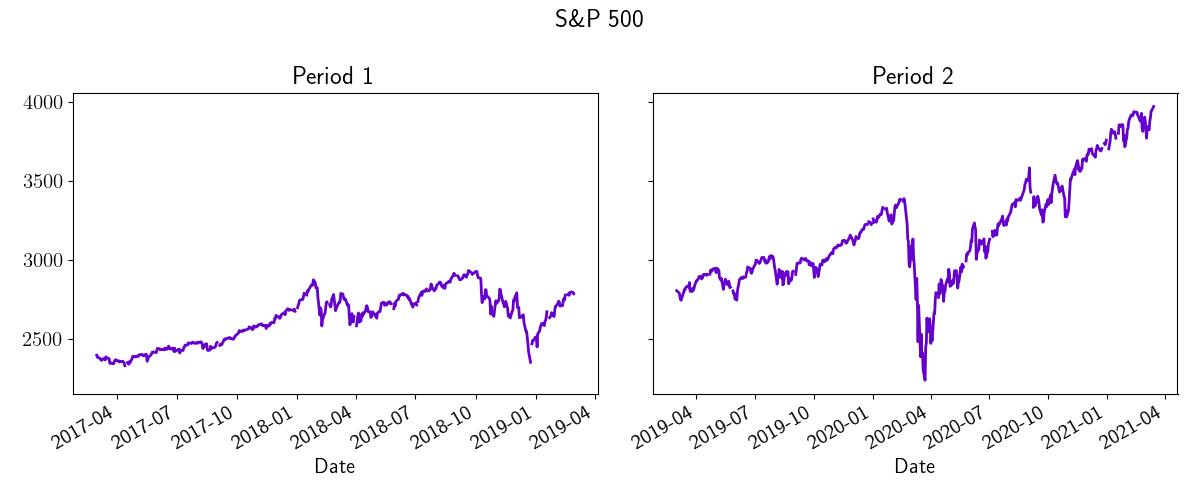
\includegraphics[width=10cm]{images/sp500.png}
s
\end{frame}


\subsection{Result}
\begin{frame}{Result}

\begin{columns}[t]

\begin{column}{0.5\textwidth}
\begin{block}{Result}
\begin{itemize}
    \item Different threshold produces portfolios with different MDD
    \item Outperformed CRP Portfolios in CAGR and MDD for most cases, 
\end{itemize}
\end{block}
\end{column}

\begin{column}{0.5\textwidth}

\begin{block}{Baseline}
Constant Rebalanced Portfolio (CRP)
\end{block}


\begin{block}{Comparison}
    \begin{itemize}
        \item CAGR
        \item MDD
    \end{itemize}
\end{block}
\end{column}


\end{columns}
\end{frame}

\begin{frame}{Result}
\begin{center}
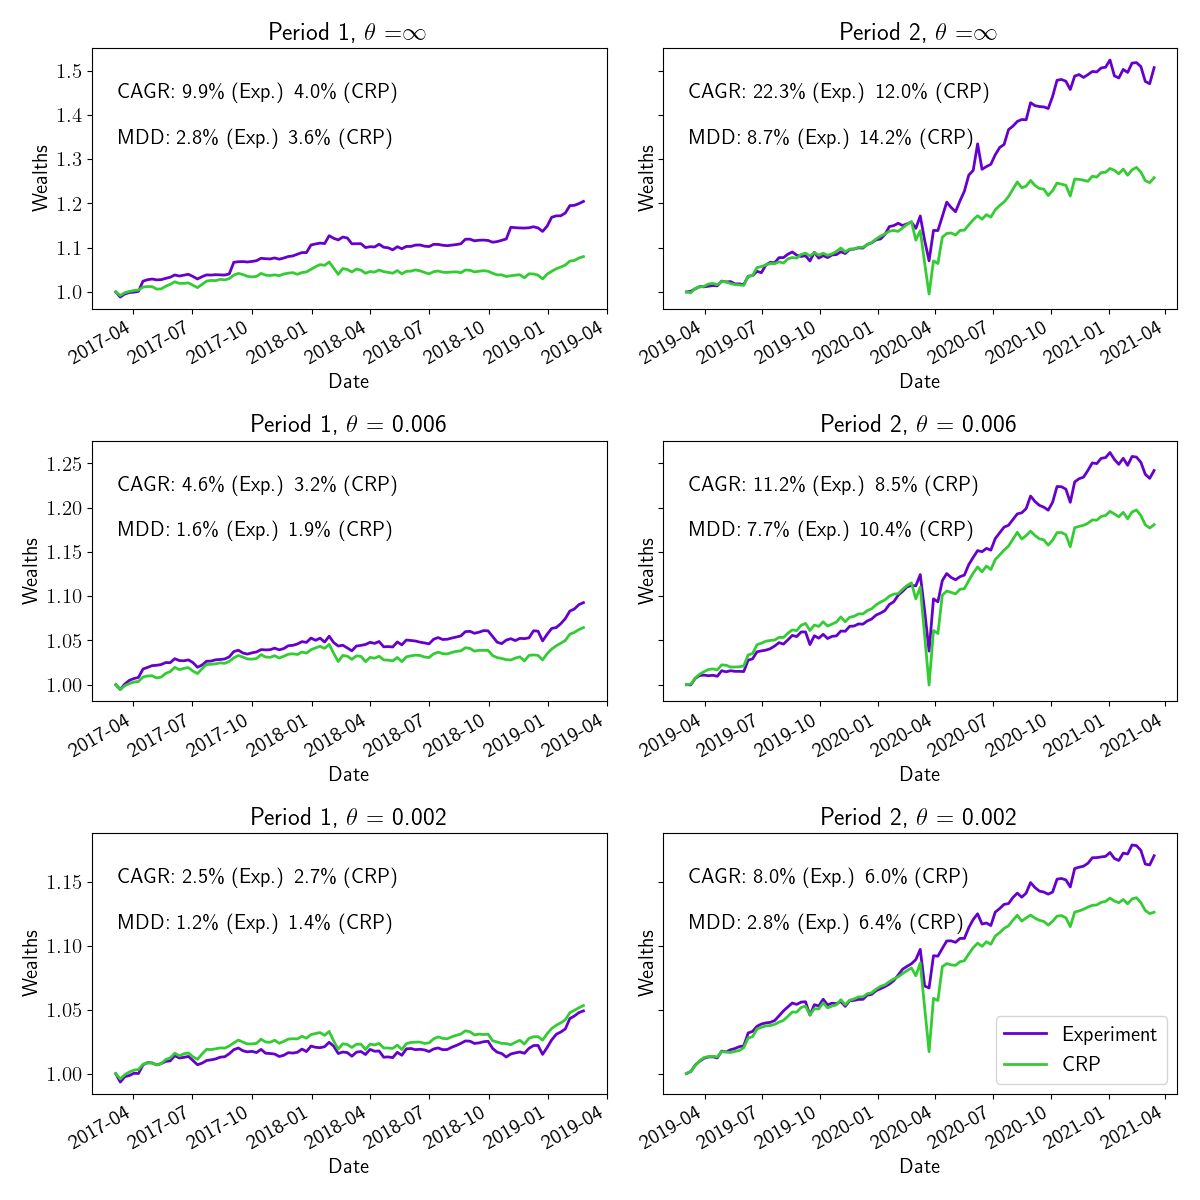
\includegraphics[height= 7.5cm]{images/crp_compare.png}
\end{center}

\end{frame}